\documentclass[11pt]{article}
\usepackage[a4paper,margin=2.4cm]{geometry}
\usepackage{amsmath,amssymb}
\usepackage{booktabs}
\usepackage{graphicx}
\usepackage[T1]{fontenc}
\usepackage{lmodern}
\usepackage{textcomp}
\usepackage{siunitx}
\DeclareSIUnit{\micrometre}{\text{\textmu}m}
\usepackage[numbers,sort&compress]{natbib}
\usepackage{lineno}
\usepackage{setspace}
\usepackage[hidelinks]{hyperref}
% Generated by make_tables.py from results_v2/summary.json -- do not edit by hand
\newcommand{\EnsN}{40}
\newcommand{\MaxOcc}{0.26}
\newcommand{\LEc}{1.43}
\newcommand{\LEcCI}{1.29--1.61}
\newcommand{\LmedEc}{1.62}
\newcommand{\LminEc}{0.74}
\newcommand{\LmaxEc}{4.02}
\newcommand{\HalfEc}{1.52 and 1.37}
\newcommand{\LSa}{1.19}
\newcommand{\LSaCI}{1.08--1.33}
\newcommand{\LmedSa}{1.35}
\newcommand{\LminSa}{0.63}
\newcommand{\LmaxSa}{3.42}
\newcommand{\HalfSa}{1.24 and 1.14}
\newcommand{\LPa}{1.45}
\newcommand{\LPaCI}{1.31--1.63}
\newcommand{\LmedPa}{1.64}
\newcommand{\LminPa}{0.73}
\newcommand{\LmaxPa}{4.02}
\newcommand{\HalfPa}{1.54 and 1.38}
\newcommand{\RhoModel}{0.83}
\newcommand{\RhoModelCI}{0.81--0.84}
\newcommand{\RhoObsA}{0.70}
\newcommand{\RhoObsCIA}{0.50--0.90}
\newcommand{\RhoPctA}{89}
\newcommand{\RhoObsB}{0.91}
\newcommand{\RhoObsCIB}{0.35--1.83}
\newcommand{\RhoPctB}{40}
\newcommand{\YobsEc}{0.118}
\newcommand{\YsdEc}{0.013}
\newcommand{\LRobsEc}{0.93}
\newcommand{\SEobsEc}{0.028}
\newcommand{\LRobsBEc}{0.79}
\newcommand{\SEobsBEc}{0.16}
\newcommand{\YobsSa}{0.224}
\newcommand{\YsdSa}{0.083}
\newcommand{\LRobsSa}{0.65}
\newcommand{\SEobsSa}{0.093}
\newcommand{\LRobsBSa}{0.72}
\newcommand{\SEobsBSa}{0.22}
\newcommand{\RhoTimeMin}{0.77}
\newcommand{\RhoTimeMax}{0.80}
\newcommand{\RhoLong}{0.86}
\newcommand{\LongEcTone}{1.72}
\newcommand{\LongSaTone}{1.36}
\newcommand{\LongPaTone}{1.67}
\newcommand{\LongEcTtt}{0.96}
\newcommand{\LongSaTtt}{0.82}
\newcommand{\LongPaTtt}{0.84}
\newcommand{\LongEcTsevtwo}{0.74}
\newcommand{\LongSaTsevtwo}{0.64}
\newcommand{\LongPaTsevtwo}{0.63}
\newcommand{\RhoPPmed}{0.74}
\newcommand{\RhoPPlo}{0.69}
\newcommand{\RhoPPhi}{0.81}
\newcommand{\RhoPPorder}{100}
\newcommand{\PaGeEc}{72}
\newcommand{\PPsnakeEc}{0.84--1.97}
\newcommand{\PPsharkEc}{1.26--1.85}
\newcommand{\PPsnakeSa}{0.62--1.52}
\newcommand{\PPsharkSa}{0.94--1.40}
\newcommand{\PPsnakePa}{0.85--1.96}
\newcommand{\PPsharkPa}{1.28--1.91}
\newcommand{\PredPaMechCI}{0.87--1.00}
\newcommand{\SharkMoreMin}{85}
\newcommand{\SharkMoreMax}{91}
\newcommand{\SharkBelowSnake}{12}
\newcommand{\Alpha}{0.64}
\newcommand{\AlphaCI}{0.56--0.72}
\newcommand{\PredPa}{0.93}
\newcommand{\PredPaCI}{0.88--0.99}
\newcommand{\PredPaRem}{0.117}
\newcommand{\PredPaRemCI}{0.103--0.133}
\newcommand{\PredPaPct}{88}
\newcommand{\LosoSa}{0.77}
\newcommand{\LosoSaCI}{0.58--0.95}
\newcommand{\LosoSaPct}{12}
\newcommand{\LosoEc}{0.79}
\newcommand{\LosoEcCI}{0.56--1.01}
\newcommand{\LosoEcPct}{89}
\newcommand{\AlphaB}{0.57}
\newcommand{\AlphaCIB}{0.37--0.77}
\newcommand{\PredPaB}{0.83}
\newcommand{\PredPaCIB}{0.55--1.09}
\newcommand{\PredPaRemB}{0.149}
\newcommand{\PredPaRemCIB}{0.081--0.284}
\newcommand{\PredPaPctB}{85}
\newcommand{\LosoSaB}{0.66}
\newcommand{\LosoSaCIB}{0.14--1.17}
\newcommand{\LosoSaPctB}{61}
\newcommand{\LosoEcB}{0.87}
\newcommand{\LosoEcCIB}{0.24--1.47}
\newcommand{\LosoEcPctB}{40}
\newcommand{\SharkEc}{1.72}
\newcommand{\SharkLateEc}{1.53}
\newcommand{\SharkAlphaEc}{0.98}
\newcommand{\SharkObsEc}{2.30}
\newcommand{\SharkSa}{1.40}
\newcommand{\SharkLateSa}{1.29}
\newcommand{\SharkAlphaSa}{0.82}
\newcommand{\SharkObsSa}{1.11--2.11}
\newcommand{\SharkPa}{1.81}
\newcommand{\SharkLatePa}{1.58}
\newcommand{\SharkAlphaPa}{1.01}
\newcommand{\SharkObsPa}{1.36--3.00}
\newcommand{\NumMean}{0.028}
\newcommand{\NumMax}{0.06}
\newcommand{\NumRel}{3}
\newcommand{\NumCoarse}{0.27}
\newcommand{\NumScreen}{0.14}
\newcommand{\NumTime}{0.0015}
\newcommand{\NumDomTwo}{0.02}
\newcommand{\NumDomFour}{0.06}
\newcommand{\NumShark}{0.15}
\newcommand{\KOTrEc}{0.62}
\newcommand{\KOTrEcCI}{0.53--0.73}
\newcommand{\KOTrSa}{0.30}
\newcommand{\KOTrSaCI}{0.24--0.37}
\newcommand{\KOTrPa}{0.67}
\newcommand{\KOTrPaCI}{0.58--0.78}
\newcommand{\KOSlEc}{0.12}
\newcommand{\KOSlEcCI}{0.09--0.15}
\newcommand{\KOSlSa}{0.08}
\newcommand{\KOSlSaCI}{0.06--0.11}
\newcommand{\KOSlPa}{0.13}
\newcommand{\KOSlPaCI}{0.10--0.16}
\newcommand{\KOApEc}{\ensuremath{-}0.04}
\newcommand{\KOApEcCI}{\ensuremath{-}0.05 to \ensuremath{-}0.03}
\newcommand{\KOApSa}{\ensuremath{-}0.01}
\newcommand{\KOApSaCI}{\ensuremath{-}0.01 to \ensuremath{-}0.01}
\newcommand{\KOApPa}{\ensuremath{-}0.05}
\newcommand{\KOApPaCI}{\ensuremath{-}0.06 to \ensuremath{-}0.03}
\newcommand{\KOCoEc}{\ensuremath{-}0.17}
\newcommand{\KOCoEcCI}{\ensuremath{-}0.20 to \ensuremath{-}0.14}
\newcommand{\KOCoSa}{\ensuremath{-}0.11}
\newcommand{\KOCoSaCI}{\ensuremath{-}0.13 to \ensuremath{-}0.09}
\newcommand{\KOCoPa}{\ensuremath{-}0.16}
\newcommand{\KOCoPaCI}{\ensuremath{-}0.18 to \ensuremath{-}0.13}
\newcommand{\KOEpsEc}{0.01}
\newcommand{\KOEpsEcCI}{0.01--0.02}
\newcommand{\KOEpsSa}{0.01}
\newcommand{\KOEpsSaCI}{0.01--0.01}
\newcommand{\KOEpsPa}{0.01}
\newcommand{\KOEpsPaCI}{0.01--0.02}
\newcommand{\KOStEc}{0.01}
\newcommand{\KOStEcCI}{0.00--0.01}
\newcommand{\KOStSa}{0.00}
\newcommand{\KOStSaCI}{0.00--0.00}
\newcommand{\KOStPa}{0.01}
\newcommand{\KOStPaCI}{0.00--0.01}
\newcommand{\DesSeedSD}{0.009}
\newcommand{\DesMinEc}{0.82}
\newcommand{\DesMaxEc}{2.71}
\newcommand{\DesLowTipEc}{0.89}
\newcommand{\DesHighTipEc}{1.54}
\newcommand{\DesNarrowEc}{1.03}
\newcommand{\DesWideEc}{1.83}
\newcommand{\DesCloseEc}{2.68}
\newcommand{\DesFarEc}{0.74}
\newcommand{\DesMinSa}{0.65}
\newcommand{\DesMaxSa}{2.09}
\newcommand{\DesLowTipSa}{0.70}
\newcommand{\DesHighTipSa}{1.10}
\newcommand{\DesNarrowSa}{0.76}
\newcommand{\DesWideSa}{1.46}
\newcommand{\DesCloseSa}{2.16}
\newcommand{\DesFarSa}{0.59}
\newcommand{\DesMinPa}{0.80}
\newcommand{\DesMaxPa}{2.74}
\newcommand{\DesLowTipPa}{0.86}
\newcommand{\DesHighTipPa}{1.59}
\newcommand{\DesNarrowPa}{1.04}
\newcommand{\DesWidePa}{1.81}
\newcommand{\DesClosePa}{2.62}
\newcommand{\DesFarPa}{0.75}
\newcommand{\STPf}{0.02--0.03}
\newcommand{\STPa}{0.77--0.82}
\newcommand{\STLen}{0.01}
\newcommand{\STBw}{0.07--0.08}
\newcommand{\STTap}{0.02}
\newcommand{\STTh}{0.18--0.22}
\newcommand{\STPitA}{0.00}
\newcommand{\STPitB}{0.00--0.01}
\newcommand{\STPitD}{0.03--0.05}
\newcommand{\STJit}{0.00--0.01}
\newcommand{\STRough}{0.03--0.04}
\newcommand{\STMinor}{0.05}
\newcommand{\KOCoMin}{0.11}
\newcommand{\KOCoMax}{0.17}
\newcommand{\KOApMax}{0.05}
\newcommand{\KOSlMin}{0.08}
\newcommand{\KOSlMax}{0.13}
\newcommand{\SMBeta}{0.30--0.31}
\newcommand{\SMcBeta}{0.06}
\newcommand{\SMAdh}{0.16--0.23}
\newcommand{\SMcAdh}{0.24}
\newcommand{\SMRng}{0.14--0.20}
\newcommand{\SMcRng}{0.17}
\newcommand{\SMTrp}{0.05--0.17}
\newcommand{\SMcTrp}{0.51}
\newcommand{\SMApp}{0.00--0.00}
\newcommand{\SMcApp}{0.00}
\newcommand{\SMAnc}{0.04--0.05}
\newcommand{\SMcAnc}{0.00}
\newcommand{\SMEpsK}{0.00--0.00}
\newcommand{\SMcEpsK}{0.00}
\newcommand{\TmT}{40}
\newcommand{\TmPa}{0.81}
\newcommand{\TmSa}{0.79}
\newcommand{\ChemLowEc}{0.27}
\newcommand{\ChemHighEc}{0.02}
\newcommand{\ChemLowSa}{0.35}
\newcommand{\ChemHighSa}{0.07}
\newcommand{\ChemLowPa}{0.23}
\newcommand{\ChemHighPa}{0.01}

\newcommand{\TITLE}{Lateral blade packing predicts bacterial retention on reconstructed ball python scales}

\newcommand{\Ec}{\textit{E.~coli}}
\newcommand{\Sa}{\textit{S.~aureus}}
\newcommand{\Pa}{\textit{P.~aeruginosa}}
\newcommand{\Preg}{\textit{P.~regius}}
\graphicspath{{../results_v2/figures/}}
\onehalfspacing
\linenumbers

\title{\TITLE}
\author{Bianca Cruz Neves$^{1}$ and Antonio Pereira$^{1,*}$\\[4pt]
\small $^{1}$Signal Processing Laboratory, Federal University of Par\'a, Bel\'em, PA, Brazil\\
\small $^{*}$Author for correspondence: apereira@ufpa.br; ORCID 0000-0002-0808-1058}
\date{}

\begin{document}
\maketitle

\begin{abstract}
\noindent Dorsal scales of the ball python (\textit{Python regius}) are covered by imbricated, tapered blades whose tips overhang small pits, and after 48~h they retain 88\% fewer \textit{Escherichia coli} and 78\% fewer \textit{Staphylococcus aureus} colony-forming units than smooth polystyrene. We reconstructed the blade array from published scanning electron micrographs and simulated how blade relief sets cell-scale contact energetics, near-surface arrival and a capacity-limited sequence of transient, anchored, matrix-producing and microcolony states, comparing each surface with a flat surface under identical physics. The \EnsN{}-reconstruction ensemble predicted weaker suppression of \textit{S.~aureus} without fitted parameters; its log-reduction ratio was \RhoModel{}, compared with \RhoObsA{} observed (95\% interval \RhoObsCIA{}). Separate grid-refinement tests on four blade arrays changed $L$ by at most \NumMax{} $\log_{10}$ units. An endpoint exponent fitted to either species predicted the other within its 95\% interval, and the same model predicted 1.4--1.8-log reductions on Sharklet AF, inside the range measured in short-term assays for two of three species. Restricted arrival between closely packed blades produced most of the suppression, and the lateral spacing between blades carried most of the geometric variance. The model predicts a 0.81--0.93-log reduction at 48~h for \textit{Pseudomonas aeruginosa} on python scales.
\end{abstract}

\noindent\textbf{Keywords:} bacterial adhesion; biomimetic surfaces; surface topography; mechanistic modelling; uncertainty quantification; Sharklet

\section{Introduction}

Microstructured surfaces suppress bacterial colonisation by controlling where cells can reach a substrate and how long they stay. Natural and engineered topographies reduce attachment, reorient cells or rupture their envelopes, and the outcome depends on feature spacing relative to cell size, on cell shape and appendages, on surface chemistry and on the stage of colonisation that an assay records \cite{Ivanova2012,Hasan2013,Wu2018,Scardino2008,Hochbaum2010,Epstein2011}. Engineered microtopographies such as the Sharklet pattern reduce colonisation by several species in short-term and biofilm assays \cite{Chung2007,May2014,Xu2017}, and combinatorial screens of thousands of polymer microtopographies have yielded statistical design rules for biofilm resistance \cite{Romero2025}. Average roughness reduces distinct feature arrangements to a single value and cannot identify which arrangement a given species will colonise.

Dorsal scales of the ball python (\Preg{}) carry a natural microtopography with a measured antibacterial effect. Scanning electron microscopy (SEM) shows imbricated, tapered protrusions up to $9.0\pm0.7$~\si{\micrometre} long whose tips are $4.6\pm0.2$~\si{\micrometre} apart along the blade axis and $4.4\pm0.6$~\si{\micrometre} apart between adjacent rows, each tip standing over a small pit in the scale sheet \cite{Peroutka2026}. Back-to-back scale pairs exposed to \Ec{} and \Sa{} for 48~h retained 88\% and 78\% fewer colony-forming units (CFU) than smooth polystyrene, cells on scales were confined to sheltered interstices between protrusions, and growth in medium containing ground skin excluded a leachable antimicrobial \cite{Peroutka2026}. Earlier metrology documented the multiscale structure of ball python skin \cite{AbdelAal2010}, and snake-inspired polymer replicas reduce colonisation by \Ec{}, \Sa{} and \Pa{} \cite{Sulochana2022}. Which features of the blade array produce suppression, and why the Gram-positive coccus escapes it more often than the Gram-negative rod, remain open.

Mechanistic models link topography to attachment at several scales. Extended DLVO theory and flow calculations relate roughness to the energy barrier and deposition rate of approaching cells \cite{Ammar2015,Hermansson1999,Bos1999}, thermodynamic models balance adhesion against envelope deformation \cite{Li2016}, molecular-dynamics and elastic-cell models resolve contact mechanics on textured surfaces \cite{Lazzini2021,Bellanato2026}, and spatial stochastic models follow attachment into early biofilm initiation \cite{Chathoth2022}. Experiments identify near-surface transport, appendage-mediated contact, the transition from reversible to irreversible adhesion and matrix production as the stages through which a cell becomes resident \cite{Zheng2021,An1998,Berne2018,Hoffman2015,Carniello2018,Dufrene2020,Jenal2017,Flemming2016,DiMartino2018,Hou2018}. Data-driven approaches learn geometry--response relations from large libraries of surfaces \cite{Tang2024,Romero2025,LeFevre2025}. The available measurements for one natural architecture and two species are insufficient to train a comparable model.

We asked whether cell-scale access to a reconstructed blade array explains the magnitude and species dependence of suppression on python scales. Each reconstructed surface was simulated alongside a flat surface under identical physics, giving a predicted remaining fraction defined in the same way as the measured CFU ratio. Measured spacings and lengths, blade widths and pit sizes estimated from published micrographs, and wide priors on unmeasured relief were propagated through an ensemble of periodic reconstructions on a verified grid. We evaluated the species contrast and leave-one-species-out predictions, then compared the Sharklet AF predictions with published short-term attachment measurements \cite{May2014,Xu2017}. Variance-based sensitivity analysis \cite{Saltelli2010} and mechanism knockouts identified the geometric features and colonisation stages that governed suppression.

\section{Material and methods}

\subsection{Observations}
Figure~5 of Peroutka et al.\ \cite{Peroutka2026} reports the 48~h assay (\Ec{} ATCC~25922 and \Sa{} ATCC~25923, three biological replicates) as CFU on scale pairs relative to polystyrene and as $\log_{10}$ CFU~cm$^{-2}$. We digitised both panels (ESM~S3). The relative values, $11.8\pm1.3\%$ and $22.4\pm8.3\%$ (mean $\pm$ s.d.), give $\log_{10}$ reductions $\mathrm{LR}_{Ec}=\LRobsEc\pm\SEobsEc$ and $\mathrm{LR}_{Sa}=\LRobsSa\pm\SEobsSa$ (s.e.), which we used throughout; the logarithmic panel gives \LRobsBEc{} and \LRobsBSa{}, and the observed species contrast and endpoint-map analyses were repeated using those values. External tests used short-term (1--4~h, static) attachment of \Ec{}, methicillin-resistant \Sa{} and three \Pa{} strains to Sharklet AF and smooth silicone \cite{May2014}, and of \Sa{} and \Pa{} to the same pattern in a second study \cite{Xu2017}, with log reductions taken from reported mean $\log_{10}$ CFU or percentage reductions (table~\ref{tab:main}).

\subsection{Surface reconstruction}
Blade arrays were represented as height fields on doubly periodic cells of about $36\times\SI{36}{\micrometre}$ (figure~\ref{fig:surfaces}a; ESM~S1). Blades sit on a lattice with following tips $p_f$ apart along the blade axis and adjacent tips $p_a$ apart in neighbouring columns offset by half a pitch. Each blade tapers from a base width $w_0$ to its tip over a projected length $\ell$ and its upper surface rises from the scale sheet to a tip height $h_t$; each tip stands over an elliptical pit that interrupts the downstream blade base. Spacings and length entered as normal priors with the reported standard deviations \cite{Peroutka2026}. Base width ($1.6$--$3.4$~\si{\micrometre}), taper and pit semi-axes were bounded by measurements on the published high-magnification micrographs, whose two-dimensional autocorrelation returned a lattice vector of \SI{4.7}{\micrometre} along the blade axis in agreement with the reported following-tip spacing. Tip height ($0.5$--$3.0$~\si{\micrometre}) and pit depth ($0.5$--$2.5$~\si{\micrometre}) cannot be measured on top-view micrographs and entered as wide uniform priors (ESM table~S3). Every random attribute of a blade depends only on its lattice index and seed, so a given blade is identical on every grid. The production ensemble contained \EnsN{} independent draws.

The Sharklet AF comparator consisted of diamond units of seven parallel ribs, \SI{2}{\micrometre} wide and \SI{3}{\micrometre} tall, 4--\SI{16}{\micrometre} long and \SI{2}{\micrometre} apart \cite{Xu2017}, tiled on a periodic $40\times\SI{32}{\micrometre}$ cell (figure~\ref{fig:surfaces}b).

\subsection{Contact, arrival and residence}
Cells and appendages sense topography over a finite length, so all geometric descriptors were computed on the height field smoothed with a Gaussian of width $\ell_s=\SI{0.25}{\micrometre}$. An effective contact cost $W$ combined short-range adhesion attenuated by the gap beneath a footprint, a compliance-reduced gap penalty, a steric penalty on relief exceeding the cell radius, a slope penalty and an appendage term that lowers the cost where appendages reach accessible surface (ESM~S1). Footprints were discs for \Sa{} and spherocylinders at four orientations for the rods, and the lowest-cost orientation was retained. The attachment propensity $p=\exp[-\beta(W-W_{\mathrm{flat}})]$ was referenced to the cost of the same species on a flat surface. Near-surface arrival $J$ fell with local slope and relief, rose with swimming speed in open regions, was smoothed over a species-specific transport length and was likewise expressed relative to its flat-surface value.

Surface-associated cells progressed through transient contact ($T$), anchoring ($A$), matrix production ($E$) and microcolony formation ($M$), supplied by a near-surface free population ($F$) replenished in proportion to $J$:
\begin{align}
\dot F&=\rho(\lambda_{\mathrm{arr}}J-F)-r_{FT}F\kappa+r_{TF}T, &\dot T&=r_{FT}F\kappa-(r_{TF}+r_{TA})T+r_{AT}A, \nonumber\\
\dot A&=r_{TA}T-(r_{AT}+r_{AE})A, &\dot E&=r_{AE}A-r_{EM}E,\qquad \dot M=r_{EM}E. \label{eq:states}
\end{align}
The free site capacity $\kappa=[1-(T+A+E+M)]_+$ stops capture as the surface fills. Capture rises with $J$ and $p$, detachment and reversion rise with slope and fall with appendage engagement, anchoring rises with $p$, and the transitions to matrix production and microcolony formation are gated by a local extracellular polymeric substance (EPS) field that is produced by $A$, $E$ and $M$, spreads through a nonlinear yield-gated diffusion term and decays (ESM~S1). The effective EPS field is dimensionless. Species coefficients combine literature-informed cell dimensions and swimming speeds with phenomenological rate and cost coefficients (ESM table~S1); they were held fixed and never fitted to the python measurements. Equations~\eqref{eq:states} were integrated with explicit Euler steps of $h=0.05$ model-time units, and the linear part of EPS spreading was advanced exactly by Strang splitting.

\subsection{Observable and endpoint map}
Retained activity $B_{\mathrm{ret}}=\langle A+E+M\rangle$, averaged over the cell at $t=4.5$ model-time units, represents firmly attached cells that survive rinsing. Each reconstruction $j$ gives a remaining fraction $Y_j=B_{\mathrm{ret},j}/B_{\mathrm{ret,flat}}$, the ensemble gives $\bar Y=N^{-1}\sum_jY_j$, the analogue of averaging CFU over specimens, and the model $\log_{10}$ reduction is $L=-\log_{10}\bar Y$. A 48~h CFU count also integrates growth and maturation, so model and observation were related by $\mathrm{LR}_s=\alpha L_s+\varepsilon_s$ with one endpoint exponent $\alpha$ shared by all species and $\varepsilon_s$ normal with the observed standard error. Because $\alpha$ multiplies both species, $L_{Sa}/L_{Ec}$ predicts $\mathrm{LR}_{Sa}/\mathrm{LR}_{Ec}$ without any fitted parameter. We estimated $\alpha$ by weighted least squares through the origin inside a Monte Carlo loop (4000 draws) that resampled reconstructions and redrew each observation from its error distribution. In leave-one-species-out tests $\alpha$ was fitted to one species and the other species' reduction was predicted with an interval that included fresh observation error. Short-term Sharklet assays record attachment within hours and were compared with $L$ at $t=1$ and $\alpha=1$.

\subsection{Numerical verification and sensitivity}
Four blade arrays and the Sharklet cell were simulated at grid spacings from 0.30 to \SI{0.07}{\micrometre}; at \SI{0.15}{\micrometre} we also halved and doubled the time step and changed the cell to 24 and \SI{48}{\micrometre}. Production runs used \SI{0.10}{\micrometre} and sensitivity screens \SI{0.20}{\micrometre}. One-at-a-time knockouts removed arrival modulation, slope cost, appendages, steric cost, compliance or EPS gating on 12 reconstructions. A design map varied tip height and base width, and a second varied adjacent-tip spacing, at three lattice seeds common to all design points. Total-order Sobol indices \cite{Saltelli2010} were estimated for the eleven geometric inputs using uniform sampling over each input's bounded support (832 geometries); these indices describe sensitivity across the specified design ranges, not variance under the truncated-normal production priors. Twelve log-uniform multipliers on mechanistic coefficients, each spanning $[1/2,2]$ and applied to all species, generated 896 coefficient sets. Bootstrap intervals used 1000 resamples. For the P. aeruginosa mechanistic-sensitivity interval, we sampled the 128 A/B coefficient settings with replacement, redrew both observed reductions from their standard-error distributions, refitted the shared endpoint exponent for each draw, and predicted the third species over 200,000 Monte Carlo draws. Because the assay compares keratin with polystyrene, controls were also simulated with body adhesion scaled by 0.8--1.25 relative to the scale surface.

\section{Results}

\subsection{Numerical accuracy}
Grid refinement from 0.10 to \SI{0.07}{\micrometre} changed $L$ by \NumMean{} on average and by at most \NumMax{}, or \NumRel\% of its value, and by at most \NumShark{} on the Sharklet cell (figure~\ref{fig:numerics}, ESM table~S4). Coarser grids underestimated suppression by up to \NumScreen{} at \SI{0.20}{\micrometre} and \NumCoarse{} at \SI{0.30}{\micrometre}, because rasterised footprints miss the narrow channels between blades. Halving or doubling the time step changed $L$ by at most \NumTime{}, and enlarging the periodic cell to \SI{48}{\micrometre} changed it by at most \NumDomFour{}. The summed surface occupancy remained below one in every reported run; no post-update clipping of total occupancy was applied (largest ensemble value \MaxOcc{}). At the production grid, the maximum discretisation change is below the experimental standard error of the \Sa{} reduction.

\subsection{Species contrast without fitted parameters}
Suppression on the reconstructed blade arrays was strong and ranked the species as observed. Ensemble log reductions were \LEc{} (95\% interval \LEcCI{}) for \Ec{}, \LSa{} (\LSaCI{}) for \Sa{} and \LPa{} (\LPaCI{}) for \Pa{} (figure~\ref{fig:ensemble}a, table~\ref{tab:main}), and every resampled ensemble placed \Sa{} below \Ec{}. The ratio $L_{Sa}/L_{Ec}$ was \RhoModel{} (\RhoModelCI{}) against an observed \RhoObsA{}, whose 95\% interval under the reported replicate dispersion is \RhoObsCIA{}; with the logarithmic panel the observed ratio is \RhoObsB{} (\RhoObsCIB{}). In the 12-reconstruction time-course subset evaluated at \SI{0.15}{\micrometre}, the ratio stayed between \RhoTimeMin{} and \RhoTimeMax{} over model times 0.5--9. An eight-reconstruction extension at the same grid spacing reached \RhoLong{} at $t=72$. Across the 128 A/B parameter settings in the Saltelli design for the twelve mechanistic multipliers, the central 90\% range of the ratio on the nominal array was \RhoPPlo{}--\RhoPPhi{}, inside the observed interval; \Sa{} was less suppressed in all 128 settings.

The weaker suppression of the coccus follows from its footprint, which fits the sheet channels left open between blades. The model places motile-cell arrival near blade crests and steep flanks, where elongated footprints rarely find low-cost orientations; the non-motile disc, subject to a weaker slope penalty, retains access to the channels (figure~\ref{fig:surfaces}c--e). Removing arrival modulation lowered $L$ by \KOTrEc{} (\KOTrEcCI{}) for \Ec{} and \KOTrPa{} for \Pa{}, compared with \KOTrSa{} (\KOTrSaCI{}) for \Sa{} (figure~\ref{fig:mechanism}a).

\begin{table}[t]
\centering
\caption{Model log reductions and the observations they predict. $L$ is the model $\log_{10}$ reduction relative to a flat surface of the same material, with a 95\% bootstrap interval over \EnsN{} blade-array reconstructions. Observed 48~h reductions on \textit{P.~regius} scales relative to polystyrene are means $\pm$ s.e.\ from three biological replicates \cite{Peroutka2026}. Predicted 48~h reductions for \textit{E.~coli} and \textit{S.~aureus} use the endpoint exponent fitted to the other species alone, with 95\% Monte Carlo predictive intervals that propagate geometry-bootstrap and observation uncertainty; the \textit{P.~aeruginosa} prediction uses the exponent fitted to both species. Sharklet AF reductions in short-term attachment assays on silicone \cite{May2014,Xu2017} are compared with $L$ at $t=1$ without any fitted parameter.}
\label{tab:main}
\small
\begin{tabular}{lccccc}
\toprule
 & \multicolumn{3}{c}{\textit{P.~regius} blade arrays, 48 h} & \multicolumn{2}{c}{Sharklet AF, 1--4 h}\\
\cmidrule(lr){2-4}\cmidrule(lr){5-6}
Species & model $L$ & observed & predicted & model & observed \\
\midrule
\textit{E.~coli} & 1.43 (1.29--1.61) & 0.93 $\pm$ 0.028 & 0.79 (0.56--1.01) & 1.72 & 2.30 \\
\textit{S.~aureus} & 1.19 (1.08--1.33) & 0.65 $\pm$ 0.093 & 0.77 (0.58--0.95) & 1.40 & 1.11--2.11 \\
\textit{P.~aeruginosa} & 1.45 (1.31--1.63) & -- & 0.93 (0.88--0.99) & 1.81 & 1.36--3.00 \\
\bottomrule
\end{tabular}
\end{table}


\subsection{Endpoint exponent and leave-one-species-out prediction}
Observed 48~h reductions were about two-thirds of the model reductions, giving $\alpha=\Alpha$ (95\% interval \AlphaCI{}; \AlphaB{} with the logarithmic panel; figure~\ref{fig:ensemble}b). The exponent fitted to \Ec{} alone predicted $\mathrm{LR}_{Sa}=\LosoSa{}$ (\LosoSaCI{}) against the observed \LRobsSa{}, and the exponent fitted to \Sa{} alone predicted $\mathrm{LR}_{Ec}=\LosoEc{}$ (\LosoEcCI{}) against \LRobsEc{}; both observations fall inside the predictive intervals, at the \LosoSaPct{}th and \LosoEcPct{}th percentiles. With $\alpha$ fitted to both species, the model predicts a 48~h reduction of \PredPa{} (\PredPaCI{}) for \Pa{}, corresponding to a remaining fraction of \PredPaRem{}. Refitting the shared exponent within each of the 128 A/B coefficient settings and redrawing the two observed reductions gave a 95\% Monte Carlo interval of \PredPaMechCI{} for the \Pa{} prediction. The two rods share motility and footprint shape, so their order varied across coefficient draws (\Pa{} more suppressed than \Ec{} in \PaGeEc\% of draws).

An exponent below one follows from the model dynamics. As accessible sites fill, retained activity on blade arrays catches up with the flat surface. In the eight-reconstruction extension, $L$ for \Ec{} fell from \LongEcTone{} at $t=1$ to \LongEcTtt{} at $t=36$ and \LongEcTsevtwo{} at $t=72$, bracketing the observed \LRobsEc{}; \Sa{} fell from \LongSaTone{} to \LongSaTtt{} and \LongSaTsevtwo{}, bracketing \LRobsSa{}. Matching model time to the 48~h endpoint through the \Ec{} reduction places it at $t\approx\TmT$. At that time, the model gives \TmSa{} for \Sa{} and \TmPa{} for \Pa{}; the endpoint-exponent map gives \PredPa{} for \Pa{}. Growth from attached cells, which the model omits, would compress the log reductions in the same direction.

\subsection{External test on Sharklet AF}
The model predicted Sharklet AF suppression in short-term assays without recalibration. At $\alpha=1$ and $t=1$ it gave log reductions of \SharkEc{} for \Ec{}, \SharkSa{} for \Sa{} and \SharkPa{} for \Pa{} (figure~\ref{fig:sharklet}, table~\ref{tab:main}). Reported reductions span \SharkObsSa{} for \Sa{} and \SharkObsPa{} for \Pa{} across strains and studies \cite{May2014,Xu2017}, enclosing both predictions, and reach \SharkObsEc{} for the single \Ec{} strain, 0.6 log above the prediction. Scaling the Sharklet predictions by the 48~h exponent would give \SharkAlphaSa--\SharkAlphaPa{} log and fall below every short-term measurement, so the two assays require different endpoint maps, as the declining model $L$ with time implies. Across the 128 A/B parameter settings in the coefficient design, Sharklet AF suppressed each species more than the nominal blade array at the same model time in \SharkMoreMin--\SharkMoreMax\% of settings, a ranking that a matched assay on both topographies can test.

\subsection{Mechanisms of suppression}
Arrival modulation produced most of the suppression for every species (figure~\ref{fig:mechanism}a). Blade crests and flanks receive fewer cells, and the remaining sheet channels are narrow relative to rod length. Slope costs added \KOSlMin{}--\KOSlMax{} log by penalising contact on flanks. Compliance and appendages lowered suppression, by \KOCoMin{}--\KOCoMax{} and by up to \KOApMax{} log respectively, because conforming envelopes and appendages restore contact with relief. Steric costs and EPS gating each changed $L$ by less than 0.02 log, because retained activity is limited by access to the surface before matrix-dependent maturation begins.

\subsection{Geometric determinants}
Adjacent-tip spacing governed suppression, with a total-order Sobol index of \STPa{} for $L$, followed by tip height (\STTh{}) and base width (\STBw{}); pit size and depth, blade length, taper, roughness and following-tip spacing each had indices of \STMinor{} or less (figure~\ref{fig:sobol}a, ESM table~S5). Closer packing narrows the sheet channels between adjacent blades, so at a tip height of \SI{1.5}{\micrometre} $L$ for \Ec{} rose from \DesFarEc{} at an adjacent-tip spacing of \SI{5.9}{\micrometre} to \DesCloseEc{} at \SI{3.4}{\micrometre}, and for \Sa{} from \DesFarSa{} to \DesCloseSa{} (figure~\ref{fig:mechanism}b--d). Taller and wider blades deepen the effect, raising $L$ for \Ec{} from \DesLowTipEc{} to \DesHighTipEc{} as tip height increased from 0.5 to \SI{3.0}{\micrometre}. The reported adjacent-tip spacing has a standard deviation of \SI{0.6}{\micrometre}, and moving across that range changes $L$ about threefold, so a more precise measurement of lateral spacing on the assayed scales would sharpen the prediction more than any other.

\subsection{Mechanistic coefficients and material chemistry}
The attachment scale $\beta$ (total-order index \SMBeta{}), body adhesion (\SMAdh{}) and adhesion range (\SMRng{}) set the magnitude of $L$, with arrival penalties contributing \SMTrp{} (figure~\ref{fig:sobol}b, ESM table~S6). The species contrast responded mainly to the strength of arrival penalties (index \SMcTrp{}) and body adhesion (\SMcAdh{}), which shift the two species' access in proportion. Across the 128 A/B parameter settings of the Saltelli design, the central 90\% range of $L$ on the nominal array was \PPsnakeEc{} for \Ec{} and \PPsnakeSa{} for \Sa{}. These settings jointly varied all twelve mechanistic multipliers, and the species contrast remained within the narrow range given above. A 20\% weaker adhesion of cells to polystyrene than to keratin would lower $L$ by \ChemLowEc{} for \Ec{} and \ChemLowSa{} for \Sa{} (ESM table~S7), so a plausible material difference corresponds to 0.2--0.35 log of the measured reductions.

\section{Discussion}

The reconstructed blade geometry provides a cell-scale account of suppression on python scales and of its species dependence. Closely packed blades leave narrow channels in the scale sheet, and the model places motile-cell arrival near blade crests and steep flanks, where elongated footprints rarely find low-cost contact orientations. The non-motile coccus retains greater access because its disc-shaped footprint fits within the channels. This spatial pattern agrees with the SEM observation that cells on scales occupy sheltered interstices between protrusions \cite{Peroutka2026}. Across the 40-reconstruction ensemble, the model reproduced the observed species ranking and log-reduction ratio without fitted parameters. The ratio remained within the observed interval in all 128 A/B settings of the joint coefficient design, and an endpoint exponent estimated from either measured species predicted the other within its predictive interval. The same contact and arrival formulation placed the \Sa{} and \Pa{} predictions within the ranges of published short-term Sharklet AF measurements.

Cell shape and size relative to feature spacing govern attachment to microtextures in experiments \cite{Scardino2008,Hochbaum2010,Wu2018}; the blade array expresses this relation through anisotropic packing. Adjacent-tip spacing dominated the geometric variance because it sets the channel width directly. Pit size and depth contributed little because the pits occupy a small fraction of the surface. Tip sharpness, central to bactericidal nanostructures \cite{Ivanova2012,Hasan2013}, enters the model through surface relief; python blades are micrometre-scale features, far larger than the nanopillars that rupture bacterial envelopes. Antifouling replicas should prioritise lateral blade packing and relief, and the design maps quantify the expected suppression across these dimensions \cite{Sulochana2022}.

The fitted endpoint exponent $\alpha=\Alpha{}$ maps the model's early-colonisation readout to a 48~h CFU count. Simulated log reductions decline as accessible sites fill. In the eight-reconstruction long-time extension, the values at $t=36$ and $t=72$ bracket the observed reductions for \Ec{} and \Sa{}. Growth from attached cells, which the model omits, would compress these differences further. This time dependence is consistent with an endpoint exponent near one for assays lasting a few hours and below one for 48~h assays. CFU ratios measured on python scales at several times would test this prediction. Single-cell measurements of reversible and irreversible adhesion \cite{Hoffman2015,Berne2018} and of mechanosensing \cite{Dufrene2020,Jenal2017} describe stages that the knockouts identify as secondary at the assumed rates. Measurements of residence times on channels and crests would test that ordering.

Material chemistry contributes alongside topography because the experimental reference surface was polystyrene. In the model, a 20\% reduction in control-surface adhesion lowers $L$ by 0.2--0.35 log units; a flat keratin control would separate this material effect from the topographic contribution. The contact, arrival and residence terms remain phenomenological, and their coefficients have not been identified experimentally. The Sobol analysis shows that coefficient variation changes the magnitude of suppression more strongly than the species contrast. The endpoint exponent maps this variation in model magnitude to the 48~h readout, while the species contrast remains comparatively stable. The surface is represented as a 2.5-dimensional height field, so cavities beneath overhanging tips enter only as pits. Flow and growth are absent from the model. The Sharklet comparison spans strains, materials and laboratories and constrains magnitudes to within about half a log. A measured \Pa{} reduction on python scales close to that of \Ec{} would support the access mechanism; a markedly different value would indicate species-specific processes beyond access.

\section*{Funding}
This work was supported by the Conselho Nacional de Desenvolvimento Cient\'ifico e Tecnol\'ogico (CNPq; grant 309589/2023-1 to A.P.) and by the Coordena\c{c}\~ao de Aperfei\c{c}oamento de Pessoal de N\'ivel Superior (CAPES).

\begin{figure}[p]
\centering
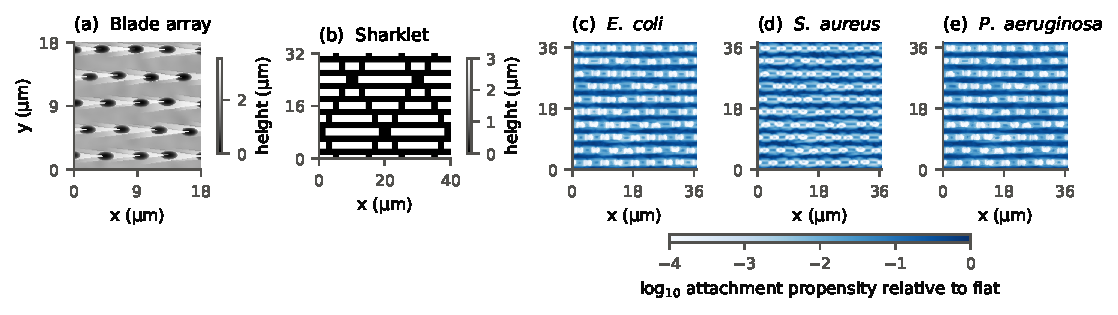
\includegraphics[width=\linewidth]{fig1_surfaces.pdf}
\caption{Reconstructed surfaces and attachment propensity. (a) An $18\times\SI{18}{\micrometre}$ window of the nominal blade array (shaded relief); blades point to the right and each tip stands over a pit. (b) Sharklet AF cell. (c--e) Attachment propensity on the nominal blade array relative to a flat surface; dark regions are favourable.}
\label{fig:surfaces}
\end{figure}

\begin{figure}[p]
\centering
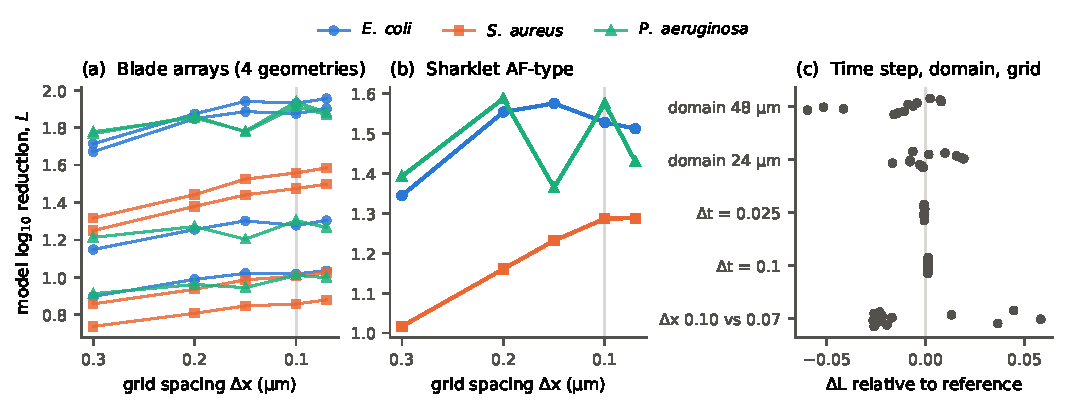
\includegraphics[width=\linewidth]{fig2_numerics.pdf}
\caption{Numerical verification. (a) Model log reduction $L$ against grid spacing for four blade arrays; the vertical line marks the production grid. (b) Same for the Sharklet cell. (c) Change in $L$ for each geometry and species when the grid is refined from 0.10 to \SI{0.07}{\micrometre}, the time step is halved or doubled, or the periodic cell is resized to 24 or \SI{48}{\micrometre}.}
\label{fig:numerics}
\end{figure}

\begin{figure}[p]
\centering
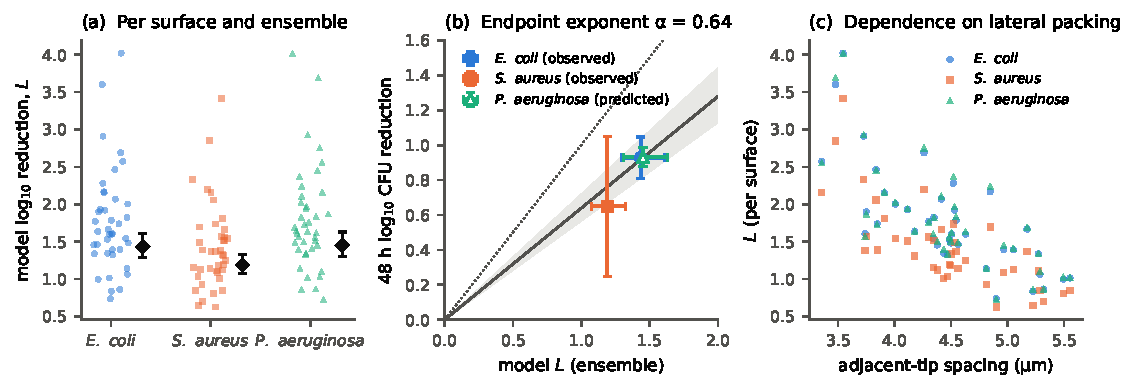
\includegraphics[width=\linewidth]{fig3_ensemble_calibration.pdf}
\caption{Ensemble predictions on python blade arrays. (a) $L$ for each of \EnsN{} reconstructions (points) and the ensemble value $-\log_{10}\bar Y$ with 95\% bootstrap interval (diamonds). (b) Observed 48~h log reductions \cite{Peroutka2026} with 95\% intervals against ensemble $L$; the solid line and band show the fitted endpoint exponent, the dotted line marks $\alpha=1$, and the open marker is the \Pa{} prediction. (c) $L$ against adjacent-tip spacing for each reconstruction.}
\label{fig:ensemble}
\end{figure}

\begin{figure}[p]
\centering
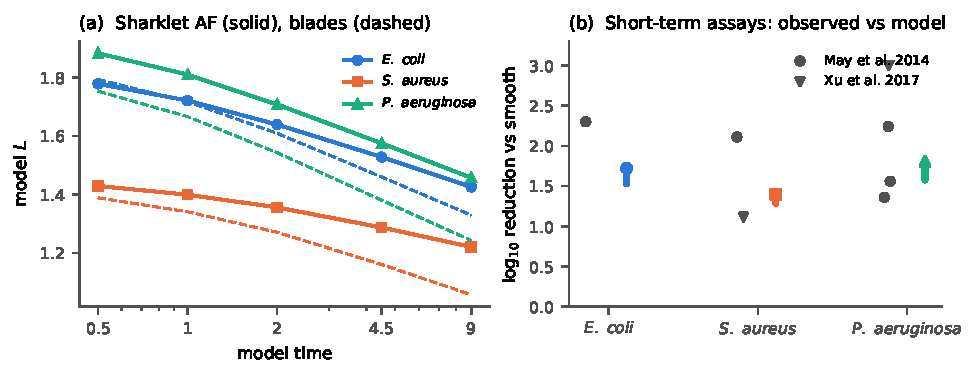
\includegraphics[width=0.9\linewidth]{fig4_sharklet.pdf}
\caption{External test on Sharklet AF. (a) Model $L$ against model time for the Sharklet cell (solid) and for 12 blade-array reconstructions (dashed). (b) Short-term log reductions on Sharklet AF relative to smooth silicone \cite{May2014,Xu2017} (grey) and model predictions with $\alpha=1$; coloured markers show $t=1$ and bars extend to $t=4.5$.}
\label{fig:sharklet}
\end{figure}

\begin{figure}[p]
\centering
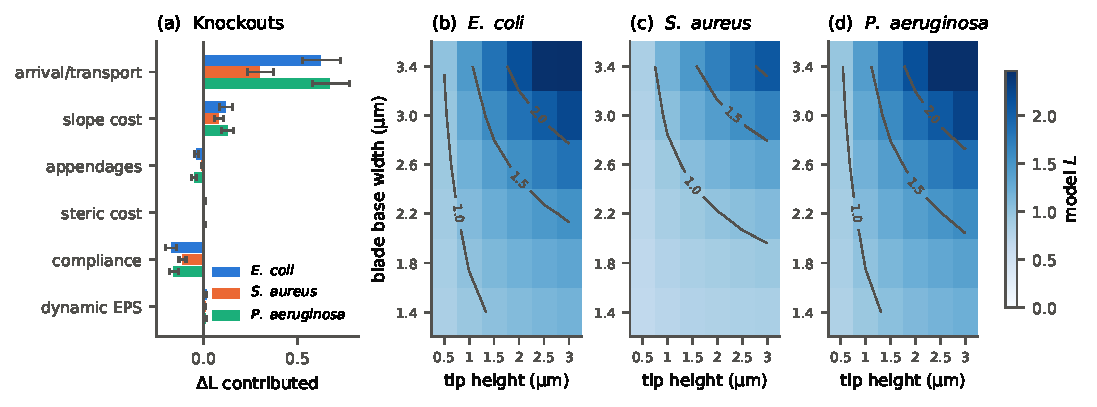
\includegraphics[width=\linewidth]{fig5_mechanism_design.pdf}
\caption{Mechanisms and design. (a) Change in $L$ when one process is removed from the full model (mean over 12 reconstructions with 95\% bootstrap interval); positive values are suppression contributed by the process. (b--d) $L$ across tip height and blade base width (mean over three common lattice seeds) with contours of $L$.}
\label{fig:mechanism}
\end{figure}

\begin{figure}[p]
\centering
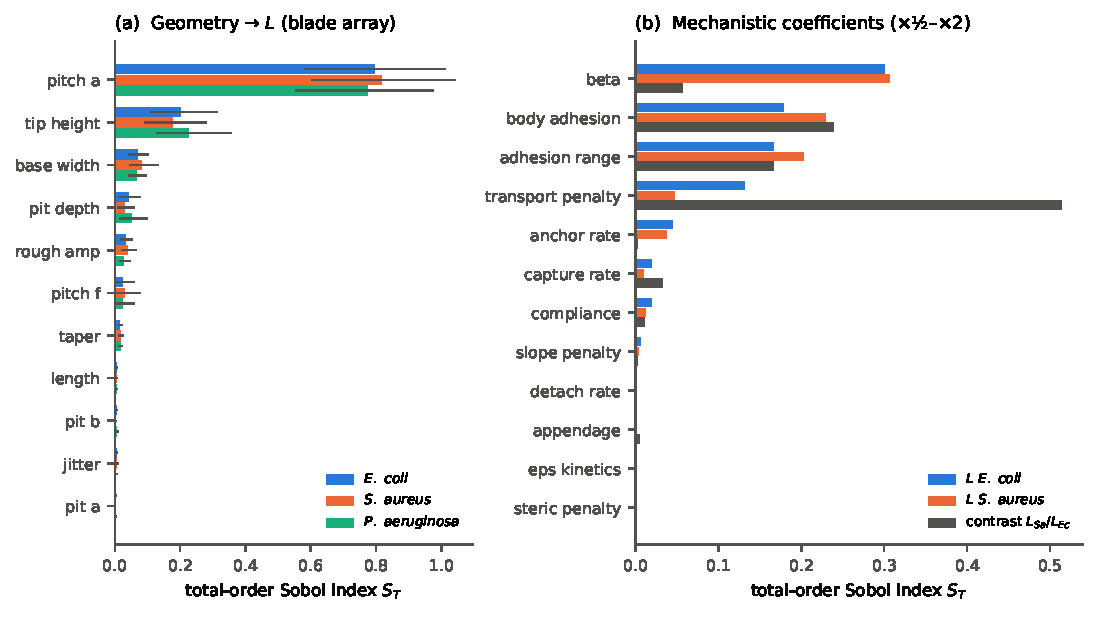
\includegraphics[width=\linewidth]{fig6_sobol.pdf}
\caption{Variance-based sensitivity. (a) Total-order Sobol indices of $L$ for the geometric inputs, with 95\% bootstrap intervals. (b) Total-order indices of multipliers on mechanistic coefficients for $L$ (\Ec{}, \Sa{}) and for the ratio $L_{Sa}/L_{Ec}$ on the nominal blade array.}
\label{fig:sobol}
\end{figure}

\clearpage
\bibliographystyle{unsrtnat}
\bibliography{refs}

\end{document}
